\subsection{Charakterisierung des Lasers auf der roten Linie}

\subsubsection{Aufbau und Durchführung}

\begin{figure}[H]
\begin{center}
  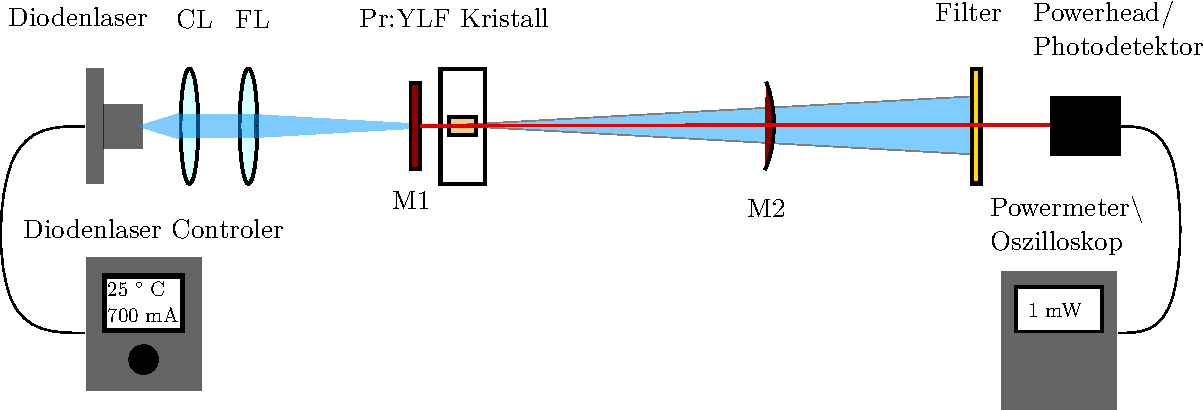
\includegraphics[width=\textwidth]{Aufbau4.pdf}
  \caption{Schematische Darstellung des Aufbaus des Lasers mit roter Linie.
  Der Aufbau ist zunächst wie in Abb.~\ref{img:aufbau3},
  allerdings benötigen wir das Spektrometer nicht und wir bauen zusätzlich einen Resonator ein.
   Direkt vor dem Kristall wird ein planer Spiegel und in knapp 10\,cm Abstand
   zu diesem hinter dem Kristall ein weiterer Spiegel mit einem Krümmungsradius von 10\,cm platziert.
   Beide Spiegel sind hoch transmittierend bei 445\,nm und hochreflektiv beschichtet bei 580-720\,nm.}
  \label{img:aufbau4}
\end{center}
\end{figure}

Für die Charakterisierung des Lasers auf der roten Linie verwenden wir den in
Abb.~\ref{img:aufbau4} dargestellten Aufbau. Die Spiegel wurden nach dem Stabilitätskriterium mit
einem Abstand von kleiner 10\,cm zuneinander um den Kristall aufgebaut. Die Spiegel wurden so
justiert, dass die Rückreflexe auf dem einfallenden Strahl liegen und nachdem durch rotieren des
Kristalls rotes Laserlicht sichtbar war wurde ihre Position auf maximale Ausgangsleistung
optimiert. Die Position des Kristalls wurde anschließend ebenfalls auf maximale Ausgangsleistung
durch drehen, kippen sowie verschieben im Fokus des Pumplasers optimiert.
Anschließend wurde zunächst mit dem OP-2 VIS Powerhead (bis 30\,mW) die Laserleistung für 25\grad
und 35\grad jeweils von 0\,A bis 1.4\,A in 50\,mA Schritten gemessen.
Anschließend wurde mit dem Photodetektor das Ausgangssignal bei 600\,mA und 25\grad bestimmt.
Zusätzlich wurde das Ausgangssignal auf einem weißen Schirm in einem Abstand von ca. 1\,m
betrachtet und dabei der hintere Resonatorspiegel leicht verkippt und mehrere Fotos der
verschiedenen Lasermoden aufgenommen.
Zur Bestimmung des dynamischen Laserverhaltens wurde das Signal mit dem Photodetektor im
modulierten Betrieb des Pumplasers bei 710\,mA und 25\grad aufgenommen. Das Signal wurde hier über
128 Perioden gemittelt.




\subsubsection{Aufnahme der Kennlinien}


\begin{figure}[H]
\begin{center}
  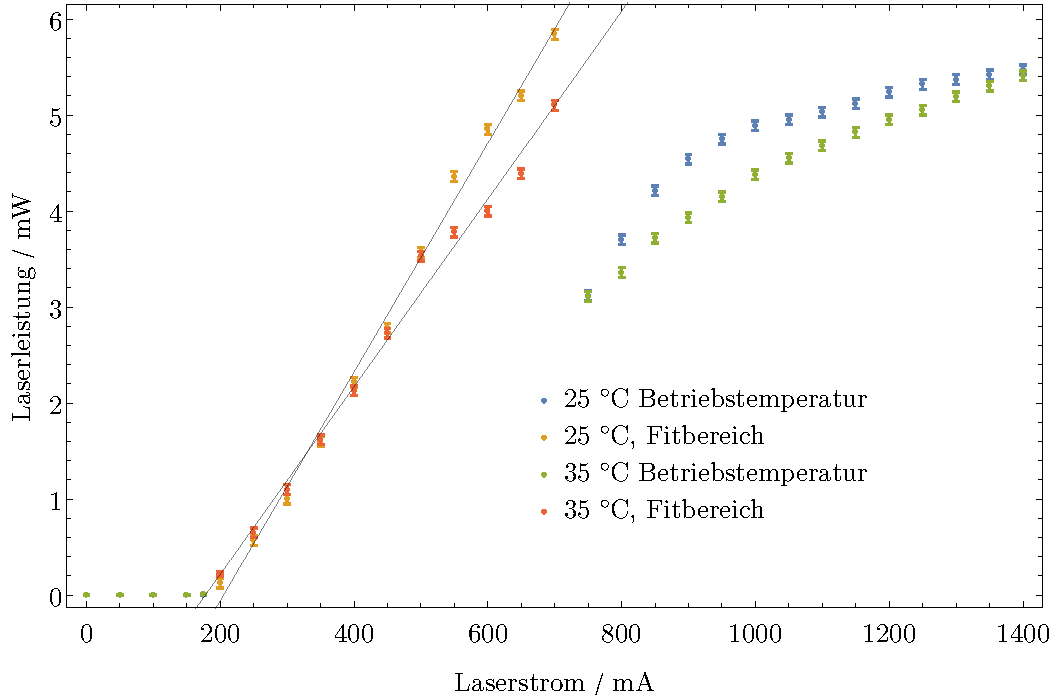
\includegraphics[width=\textwidth]{PI_rot.pdf}
  \caption{PI-Kennlinie des roten Lasers bei 25\grad und 35\grad
  Betriebstemperatur. Der modulationsfreie Bereich wurde mit $y=a(x-b)$
  gefittet, um die Laserschwelle~$b$ und die Effizienz~$a$ zu bestimmen.}
  \label{img:PI_rot}
\end{center}
\end{figure}


\begin{table}[htb]
\caption{Ergebnisse der Fits der PI-Kennlinien roten Lasers mit $y=a(x-b)$ von 200\,mA bis
700\,mA Laserstrom.}
\begin{center}
\begin{tabular}{|c|c|}
\hline
\textbf{25\grad} &  \\ \hline
$a$ & 11.91\,$\pm$\,0.10\,\textmu W\,/\,mA \\ \hline
$b$ & 204.9\,$\pm$\,2.3\,mA \\ \hline
\textchi$^2$ & 79.2873 \\ \hline
\textchi$^2$/\,DoF & 8.8097 \\ \hline
 &  \\ \hline
\textbf{35\grad} &  \\ \hline
$a$ & 9.77\,$\pm$\,0.07\,\textmu W\,/\,mA \\ \hline
$b$ & 177.7\,$\pm$\,1.9\,mA \\ \hline
\textchi$^2$ & 101.847 \\ \hline
\textchi$^2$/\,DoF & 11.3164 \\ \hline
\end{tabular}
\end{center}
\label{tab:Fits_PI_rot}
\end{table}

\FloatBarrier

\subsubsection{Messung der Laserleistung mit Photodiode}



\subsubsection{Erzeugung verschiedener Moden}


\subsubsection{Messung des dynamischen Verhaltens}

\begin{figure}[H]
\begin{center}
  \includegraphics[width=.7\textwidth]{LaserEinschwingvorgang.png}
  \caption{Photodiodenspannung (blau) nach Einschalten der Laserspannung (gelb).
  Ein dynamisches Einschwingen der Laserintensität ist erkennbar.}
  \label{img:Einschwingen}
\end{center}
\end{figure}